\section{Installing and Configuring Cardano Development Tools}\label{sec:setup}
The purpose of this book is to gather all the information for developing on Cardano that currently is scattered around.
What are we going to use for our project?


\begin{itemize}
    \item \textbf{A hot Wallet}: We are going to use a wallet to test our contracts, this wallet will be used in to receive tADA. We'll never store our main ADA holdings in this wallet: Wallets reccomended for testnet are Nami on desktop and  Vespr for mobile.
    \item \textbf{A indexer account}: Indexers are the ones that will provide us the APIs in order to interact with the chain, we won't need to run a node for testing, let's use services and projects already there like \textbf{Maestro}, let's setup an account and get the API key.
    \item \textbf{Lucid library}: Lucid is not mantained anymore as function and has being replaced by COMING SOON, however for testing and understanding the flow of Cardano transactions it can be really useful.
    \item \textbf{tADA}: How are we going to test without having testnet ADA? let's not mess up real ADA
    \item  \textbf{IDE}: Personally I use Visual Studio Code as IDE, but any other editor is ok since we are going to 
    \item \textbf{Cardano Node:} This is NOT mandatory at all, however as homework we could try to setup a cardano node and interact with the chain using cardano-cli (command line), however this is something we can do in our free time, there are other hobbies out there better than this, swimming, dancing or reading a book.
\end{itemize}

\section{Setting Up and Connecting to Cardano Testnet}
So let's install a wallet and config for testnet 

In this example we'll install Nami wallet that we can find \href{https://www.namiwallet.io/}{here}

Once we install the wallet we'll get 24 seed phrase words

\begin{remark}
Never share the seedphrase or store it on a cloud, use a paper or different ways to store, software can keep track of your seedphrase and you could lose the funds.
\end{remark}

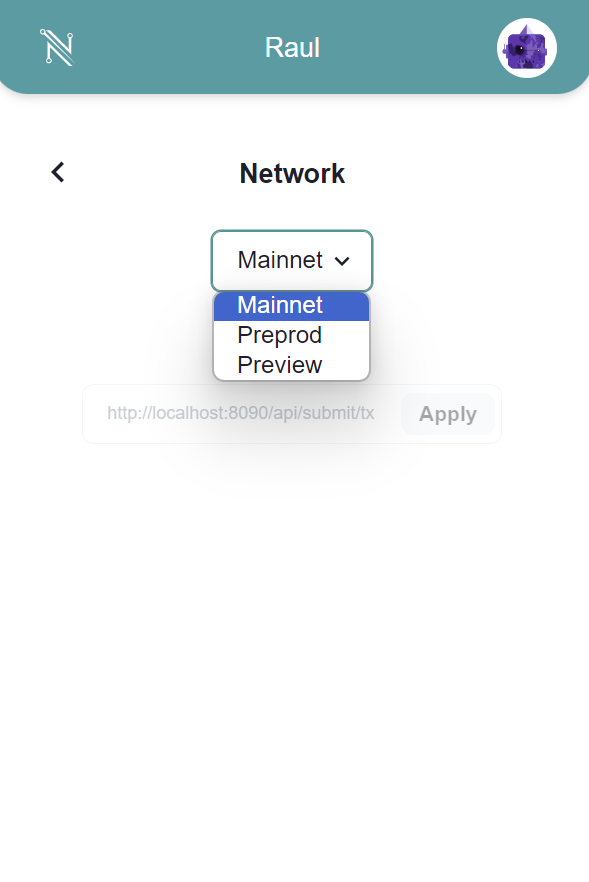
\includegraphics{wallet_preview}

Let's set Nami to \textbf{testnet preview} and we'll finally get our wallet in testnet 

In order to receive tADA we can use the official faucet from Cardano at the following \href{https://docs.cardano.org/cardano-testnets/tools/faucet/}{link}

\subsection{CIP30}

In order to connect our wallet with any webpage we'll use CIP30 reference, we can find the list of methods to connect and invoke the functions of the wallets at this \href[https://www.cardano-caniuse.io/]{page}

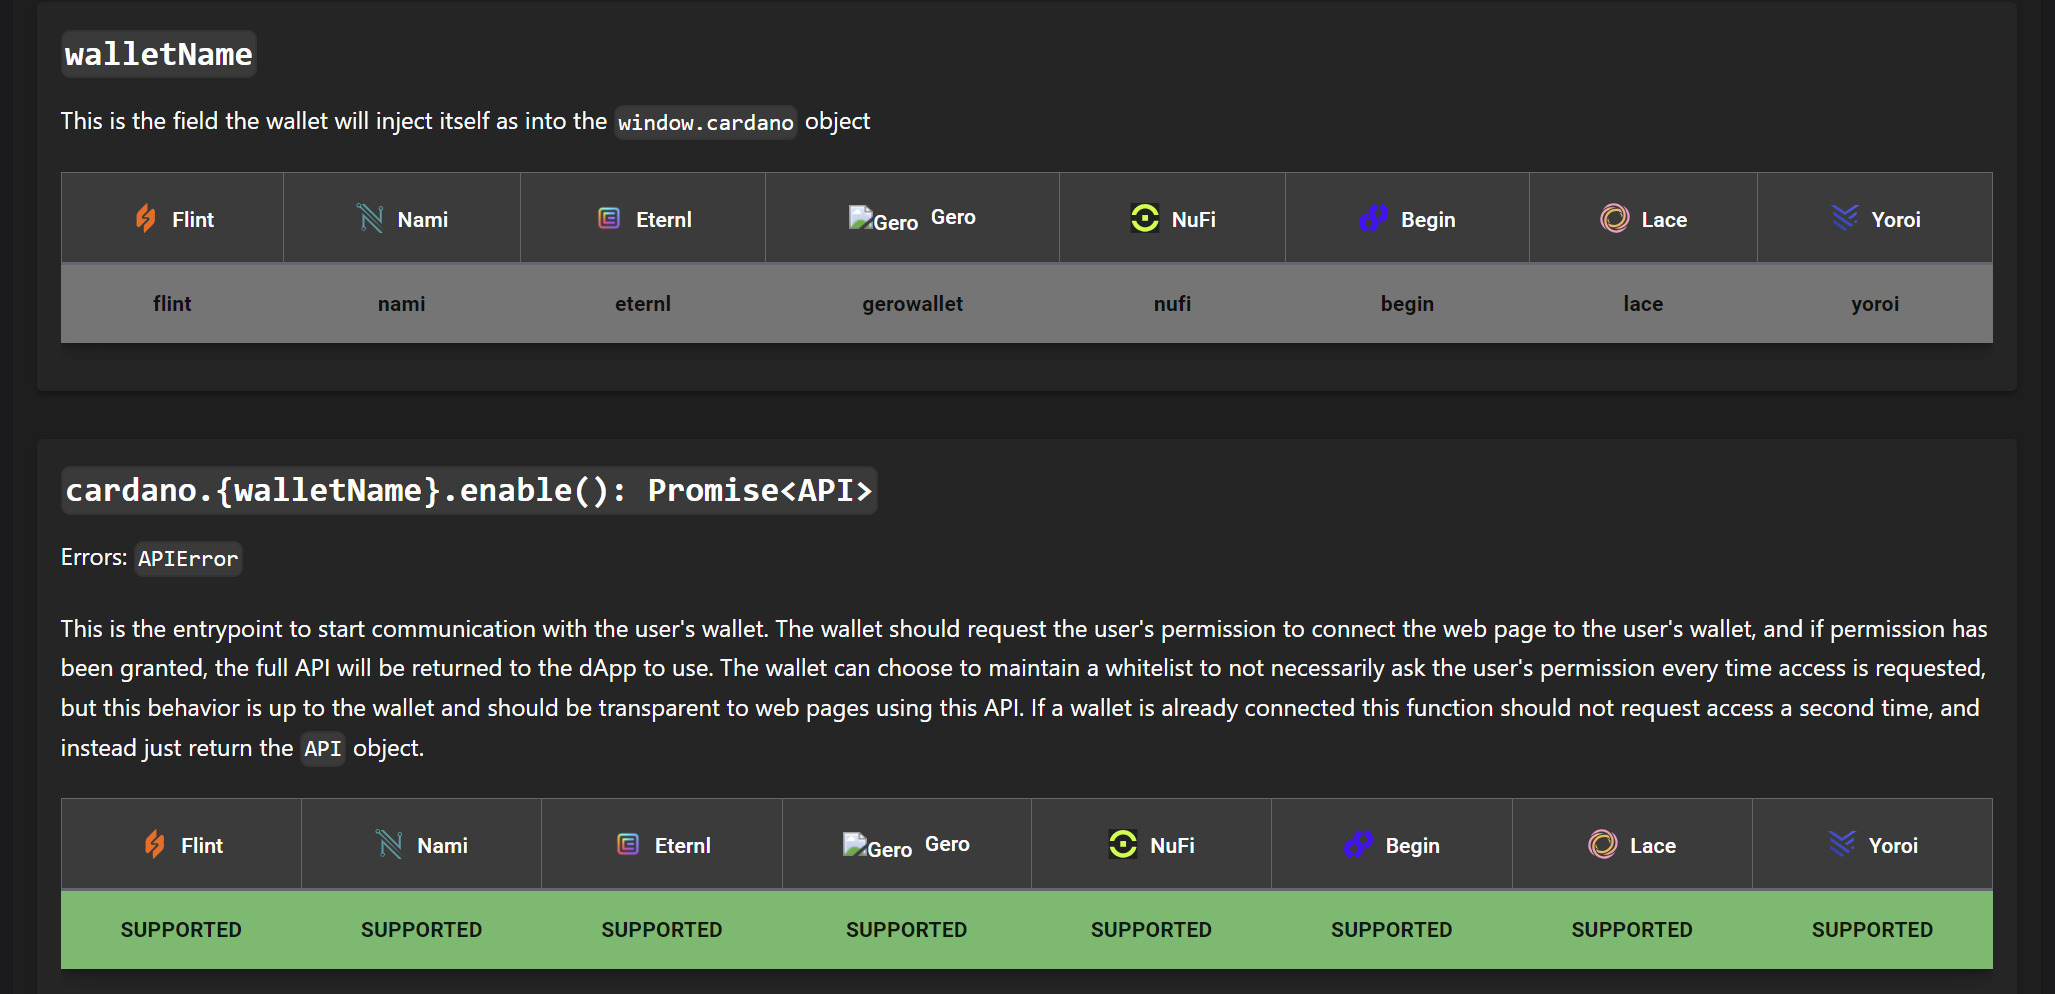
\includegraphics[scale=0.5]{cip30}

The steps to interact with a wallet following cip30 are:

\begin{itemize}
    \item \textbf{cardano.{walletName}.enable()}: we get an API object as promise, this will create a popup message to allow the wallet to connect to the current website
    \item \textbf{api.getBalance()}:using the api object we got before, we get the total amount of lovelace in the wallet (1 ADA = 1000,000 lovelace)
    \item \textbf{api.signTx}: Signing a tx that was build with Lucid or any other library we sign and interact with the blockchain 
\end{itemize}

\begin{remark}
    EXCERCISE 1: Create a webpage with 2 butttons, 1 to enable the wallet connection, second button to view the amount of ADA in the wallet.
\end{remark}


\section{Interacting with Cardano Node and Wallet APIs}

CIP30 is not enough, what if we want to get the informations regarding a specific NFT in our wallet?
How to get the list of tokens inside the wallet and get information regarding their circulation supply?

We need an indexer. We could setup one on our own or use a service, in this book we'll use \textbf{Maestro} as service provider so the first thing to do is:

\subsection{Create a Maestro account}

Head over \href{https://dashboard.gomaestro.org/login}{Maestro login} page and create an account, here we'll be able to get the API keys to interact with Cardano.

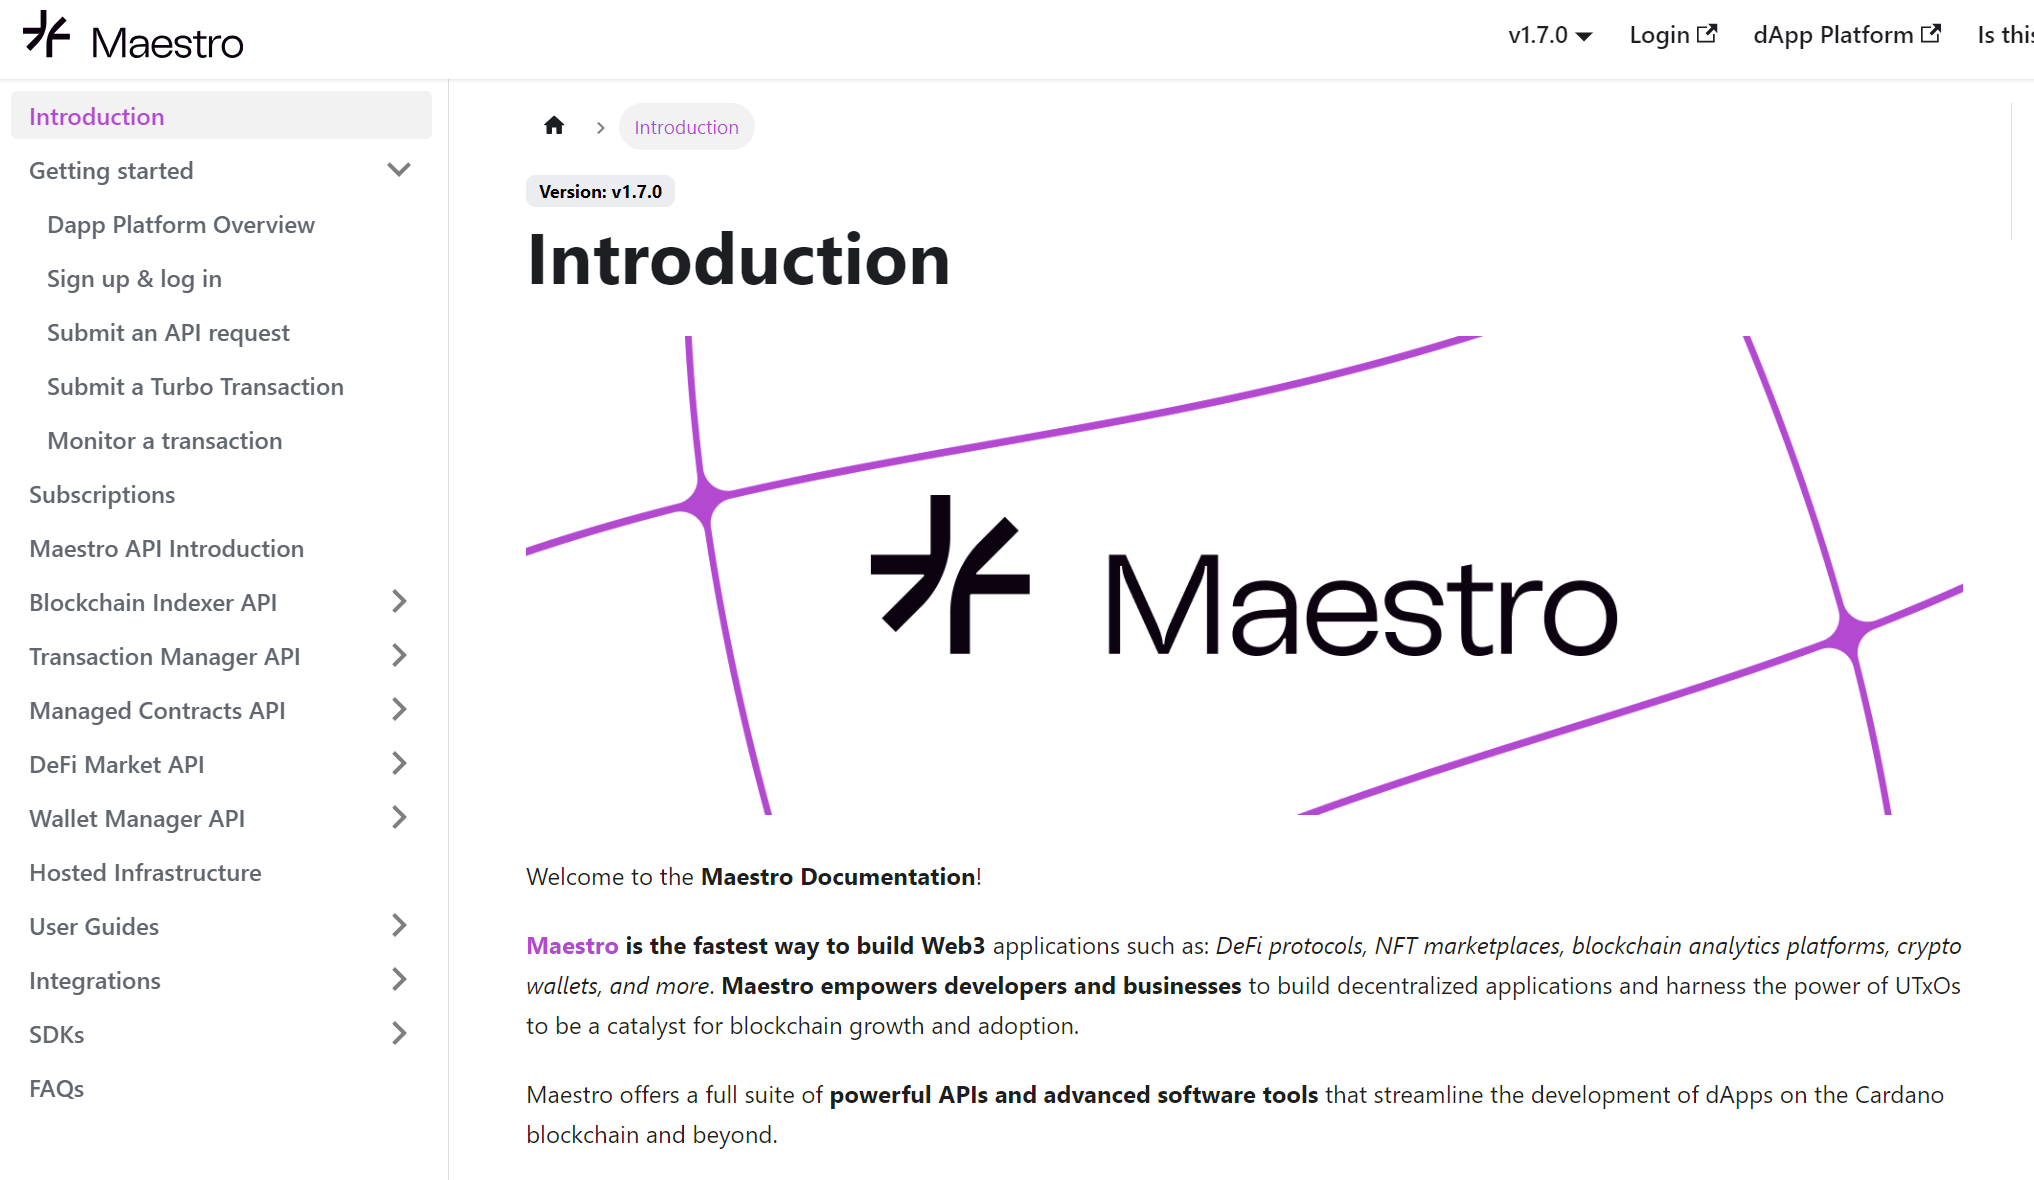
\includegraphics[scale=0.5]{maestro.png}

Maestro is going to be our key to get all the possible APIs in order to interact with Cardano, here the possible things we can do with these APIs:

\begin{itemize}
    \item Get the history of an address with this \href{ttps://docs.gomaestro.org/Indexer-API/Addresses/txs-by-address}{API}
    \item Get all the assets of a specific policy 
    \item Get the address holding a specific ada handle
    \item Get the history of holders for a specific NFT 
    \item and much more 
\end{itemize}

Now that we have a way to interact with a wallet and APIs to query the Cardano blockchain we are ready to put our hands on the real coding part.

Let's code smart contracts.

\begin{remark}
    EXCERCISE 2: Head over http://cnftlab.party/ and connect your testnet wallet, mint a collection of NFTs and then use Maestro to get the information of each NFT of your collection.
\end{remark}


